%% Application of overlap model to molecules like Cl2, F2, N2:
%% \cite{Wheatley1990}

%% More complicated atomic density partitioning by Mitchell and Price:
%% \cite{Mitchell2000}

%% Study of heteroatomic species, confirmation of model for homoatomic and
%% jellyium species:
%% \cite{Ihm1990}
%% 
%% Overlap model for inert gas atoms, suggestion of $S^2/R$ term, combing rules for
%% mixed systems:
%% \cite{Nyeland1986}`
%% 
%% Overlap model (both orbital and density) for EFP methods:
%% \cite{Soderhjelm2006}
%% 
%% Molecule justification for overlap model:
%% \cite{Wheatley1990,Mitchell2000,Soderhjelm2006}

%% Add (and read) Overlap Model Papers: see refs 23, 38-46 in \cite{Day2003};
%% check with Alston and Anthony for what they know about this.

We begin with a formal treatment of the overlap model for the
exchange-repulsion between two isolated atoms, and then extend 
these results to develop a generalized model for the short-range 
interactions in both atomic and molecular systems. 
Finally, we show how the conventional Born-Mayer model can be derived as an
approximation to this more rigorous treatment.

\begin{subsection}{Models for the exchange-repulsion between isolated atoms}
\label{sec:isotropic-homoatomic_vrep}

It is well known that the exchange-repulsion interaction between two
closed-shell atoms $i$ and $j$ is proportional, or very nearly proportional, 
to the overlap of their respective charge densities:
\cite{Kim1981}
%
\begin{gather}
\label{eq:isotropic-atomic_vrep}
%\begin{split}
\erep_{ij} \approx \vrep_{ij} = K_{ij}(S_{\rho}^{ij})^{\gamma} \\
\label{eq:isotropic-overlap}
S^{ij}_{\rho} = \int \rho_i(\mathbf{r}) \rho_j(\mathbf{r}) d^3\mathbf{r}.
%\end{split}
\end{gather}
%
Here and throughout, we use $E$ to denote quantum mechanical energies,
and $V$ to denote the corresponding model/force field energies.
Recently two of us have
provided a theoretical justification for this repulsion hypothesis (or overlap
model), and have shown that
$\gamma=1$ provided that asymptotically-correct densities are used to
compute both the atomic densities and $\erep_{ij}$.\cite{Stone2007,Misquitta2015a} 
As this is the case for the calculations in this work, we assume $\gamma=1$
throughout the Chapter.

The overlap model has frequently been utilized in the literature
and has been found to yield essentially quantitative accuracy for a wide variety of
chemical systems.\cite{Kim1981,Nyeland1986,Ihm1990} 
Prior work exploiting the overlap model has generally followed
one of two strategies. Striving for quantitative accuracy, several
groups have developed approaches to evaluate \cref{eq:isotropic-overlap}
via either numerical integration or density fitting of ab-initio molecular
electron densities, $\rho_{i}$ (e.g. SIBFA, GEM, effective fragment potentials).
\cite{Duke2014,Elking2010,Cisneros2006a,Chaudret2014,Chaudret2013,Ohrn2016,
Gresh2007,Gordon2001,Xie2007,Xie2009}
%CITE: SIBFA, X-pol, EFP, etc.
These force fields, while often extremely accurate, lack the simple closed-form analytical expressions that
define standard force fields (such as the Lennard-Jones or Born-Mayer models) and thus are often
much more computationally expensive than conventional models.

In contrast, and similar to our objectives, the overlap model has also been used in the development of standard
force fields. In this case, the molecular electron density as well as the overlap
itself is drastically simplified in order to yield a simple closed-form
expression that can be used within a conventional molecular simulation package.
\cite{Kim1981,Nyeland1986,Ihm1990} 
As we show below, the Born-Mayer model can be `derived' via such an approach.  At the expense of some accuracy, the resulting
overlap-based force fields exhibit high computational efficiency and employ well-known functional forms.

Building on this prior work, our present goal
is to derive rigorous analytical expressions and improved approximations for
both $\rho_{i}$ and \cref{eq:isotropic-overlap}, facilitating the construction of ab initio force fields
that exhibit simplicity, high computational efficiency, fidelity to the underlying PES, and (with only trivial modifications) compatibility with standard simulation packages.
%
We first start with the case of isolated atoms, where it is well-known that the
atomic electron density decays asymptotically as
%
\begin{align}
\rho_{r \to \infty}(r) \propto r^{2\beta} e^{-2\alpha r}
\end{align}
%
where the exponent $\alpha = \sqrt{2I}$ is fixed by the vertical ionization potential
$I$, $\beta= -1 + \frac{Q}{\alpha}$, 
and $Q=Z-N+1$
for an
atom with nuclear charge $+Z$ and electronic charge $-N$.
\cite{PatilT-AsymptoticMethods,Hoffmann-Ostenhof1977,Amovilli2006,Misquitta2015a}
The exponential term dominates the asymptotic form of the density,
and the $r$-dependent prefactor may be neglected \cite{Nyeland1986, Ihm1990, Bunge1986, Misquitta2014}.
In this case, the density takes the even simpler form
%
\begin{align}
\label{eq:isotropic-rho_tail}
\rho_{r \to \infty}(r) \approx De^{-B r},
\end{align}
%
where $D$ is a constant that effectively absorbs the 
missing $r$-dependent pre-factor and $B$ is an exponent that is now only approximately equal to 
$2\alpha$. 

In the case of two identical atoms, 
substitution into \cref{eq:isotropic-overlap} yields a simple expression for the density overlap, $S_{\rho}$,
\cite{Tai1986,Rosen1931}
%
\begin{align}
\label{eq:isotropic-simple_overlap}
\begin{split}
S^{ii}_{\rho} = \frac{\pi D^2}{ B^{3}} P(B r_{ii}) \exp(-B r_{ii}) \\
P(B r_{ii}) = \frac13 (B r_{ii})^2 + B r_{ii} + 1 
\end{split}
\end{align}
%
as well as (via \cref{eq:isotropic-atomic_vrep}) the exchange-repulsion energy\cite{Ihm1990,Rappe1992}:
%
\begin{align}
\label{eq:isotropic-homoatomic_vrep}
\vrep_{ii} = \Aex{ii} P(B r_{ii}) \exp(-B r_{ii}).
\end{align}
%
Here, $r_{ii}$ represents an interatomic distance, and $\Aex{ii}$
indicates a proportionality constant that is typically fit to calculated
values of the exchange-repulsion energy. The only approximations thus far
are the use of the overlap model and the simplified asymptotic form of 
the atomic charge density.
%

%% \end{subsection}
%% \begin{subsection}{Exchange-Repulsion for Atoms}
%% \label{sec:isotropic-heteroatomic_vrep}


For the general case of two hetero-atoms, substitution of
\cref{eq:isotropic-rho_tail} into \cref{eq:isotropic-overlap} yields the more complicated expression
\cite{Tai1986,Rosen1931}
\begin{align}
\label{eq:isotropic-complicated_overlap}
\begin{split}
S^{ij}_{\rho} = &
\frac{16\pi D_i D_j \exp(-\{B_i + B_j\}r_{ij}/2)}{(B_i^2-B_j^2)^3r_{ij}}
\times \\
\Bigg [ &
\left(\frac{B_i - B_j}{2}\right)^2 
\bigg(\exp \left(\{B_i-B_j\}\frac{r_{ij}}{2}\right) - \exp \left(-\{B_i-B_j\}\frac{r_{ij}}{2}\right) \bigg) \\
& \qquad \times \left( \left(\frac{B_i + B_j}{2}\right)^2r_{ij}^2 + (B_i + B_j)r_{ij} + 2 \right) \\
& - \left(\frac{B_i + B_j}{2}\right)^2 \exp \left(\{B_i-B_j\}\frac{r_{ij}}{2}\right)
\times \left( \left(\frac{B_i - B_j}{2}\right)^2r_{ij}^2 - (B_i - B_j)r_{ij} + 2 \right) \\
& + \left(\frac{B_i + B_j}{2}\right)^2 \exp \left(-\{B_i-B_j\}\frac{r_{ij}}{2}\right)
\times \left( \left(\frac{B_i - B_j}{2}\right)^2r_{ij}^2 + (B_i - B_j)r_{ij} + 2 \right)
\Bigg ],
\end{split}
\end{align}
%
which is too
cumbersome to serve as a practical force field functional form.
However, since the above expression reduces to
\cref{eq:isotropic-simple_overlap} in the limit $B_i = B_j$, 
and because $|B_i - B_j|$ is small for most atom pairs,
we have found that \cref{eq:isotropic-complicated_overlap} may be approximated
using \cref{eq:isotropic-simple_overlap} with an \emph{effective} atomic exponent $B$. 
An expansion of \cref{eq:isotropic-complicated_overlap} about $B_i = B_j$
suggests that this effective exponent should be given by the arithmetic mean,
$\B = \frac12 (B_i + B_j)$. However, a Waldman-Hagler style analysis \cite{Waldman1993}
(\cref{sec:bij_combo_rule}) suggests instead that a more suitable
exponent is given by the geometric mean combination rule,
%
\begin{align}
\label{eq:isotropic-isaff_bij}
B = \B \equiv \sqrt{B_iB_j}.
\end{align}
% 
As shown in the \si of \citen{VanVleet2016}, this approximate overlap model (\cref{eq:isotropic-simple_overlap} and
\cref{eq:isotropic-isaff_bij}) is of comparable accuracy to the exact overlap from 
\cref{eq:isotropic-complicated_overlap}. 
Thus the density overlap and (force field) exchange energies of arbitrary hetero-atoms
take the simple forms
%
\begin{align}
\label{eq:isotropic-isaff_overlap}
S^{ij}_{\rho} &= D_{ij} P(B_{ij}, r_{ij}) \exp(-B_{ij}r_{ij}) \\
D_{ij} &= \pi D_i D_j B_{ij}^{-3} \\
P(B_{ij},r_{ij}) &= \frac13 (B_{ij} r_{ij})^2 + B_{ij} r_{ij} + 1
\end{align}
%
and
%
\begin{align}
\label{eq:isotropic-isaff_vrep}
\vrep_{ij} = A^{exch}_{ij} P(B_{ij} r_{ij}) \exp(-B_{ij}r_{ij}).
\end{align}
%
Due to the connection with the overlap between two s-type Slater orbitals, we refer
to \cref{eq:isotropic-isaff_vrep} as the Slater functional form. Note that this expression reduces
to the standard Born-Mayer function by making the further approximation $P(B_{ij}
r_{ij}) = 1$, although it is known\cite{Ihm1990, McDaniel2012} that 
this is a poor approximation with the $B_{ij}$ as defined above.
Instead, as we shall demonstrate in \cref{sec:isotropic-results}, the
exponents \B need to be scaled for accurate use with a Born-Mayer functional form.

Variants of the polynomial
pre-factor from \cref{eq:isotropic-isaff_overlap} have previously been recognized and
used in intermolecular interaction models.
\cite{Buckingham1938,McDaniel2012,Rappe1992}
Early work by \citeboth{Buckingham1938} hypothesized that the functional form
of \cref{eq:isotropic-isaff_vrep} would be more accurate than the Born-Mayer
form, though no attempt was made to provide a closed-form expression for
$P$. More recent potentials have incorporated a low-order
polynomial into the exchange repulsion term, either by direct parameterization
\cite{Podeszwa2006, Bukowski2006, Jeziorska2007, Sum2002, Konieczny2015} 
or indirectly by fitting the exchange to ${S_{\rho}}/{r^2}$ rather than
to $S_{\rho}$ itself.
\cite{Kita1976a,Nyeland1986,Ihm1990}
\citeauthor{Kita1976a} have derived (but not tested) \cref{eq:isotropic-homoatomic_vrep} for
the homoatomic case.
\cite{Kita1976a}
Recently, and most similar to the spirit of the present Chapter,
York and co-workers have derived a model based upon the overlap of Slater-type orbitals
for use in QM/MM simulations, yielding an expression identical to
\cref{eq:isotropic-complicated_overlap}.
\cite{Kuechler2015,Giese2007,Giese2013} 
Those authors treated $D_i$ and $D_j$ as empirical fitting
parameters and estimated atomic exponents ($B_i$ and $B_j$) via atomic-charge dependent functions.
In contrast, we will demonstrate that utilization of the far simpler
functional form from \cref{eq:isotropic-isaff_vrep},
in conjunction with exponents calculated from analysis of the first-principles molecular electron density,
yields much higher computational efficiency and simplifies the
parameterization process without significant loss of accuracy.

%% We believe that we are the first to provide a simple and general closed-form
%% expression for both $P$ and $\vrep_{ij}$ that requires no additional
%% parameterization compared to the Born-Mayer model and is (\emph{vide infra})
%% amenable to the simple combining rules typical of standard force fields.

For an arbitrary pair of interacting atoms, $\Aex{ij}$ can be obtained by
fitting to calculated exchange-repulsion energies. However, assuming that the
overlap proportionality factor $K_{ij}$ is a universal
constant (or, alternatively, separable 
with $K_{ij} = K_iK_j$), then 
\begin{align}
\label{eq:isotropic-isaff_aij}
\Aex{ij} = \left(K_i\sqrt{\frac{\pi}{B_i^3}}D_i\right)
\left(K_j\sqrt{\frac{\pi} {B_j^3}} D_j\right) \equiv \Aex{i}\Aex{j},
\end{align}
%
thus providing a combination rule for heteroatomic interaction in
terms of purely atomic quantities. The universality and separability
of $K_{ij}$ are, at present, empirically rather than theoretically justified.
\cite{Day2003,Stone2007,Nobeli1998}
The $\Aex{i}$ can then be obtained, for
example, by a straightforward fitting of calculated ab initio
\emph{homoatomic} exchange-repulsion energies.

\end{subsection}
\begin{subsection}{Models for other short-range interactions between isolated atoms}
\label{sec:isotropic-heteroatomic_vsr}

Beyond the exchange-repulsion, the density-overlap model may also be used
to model other short-range interaction components, such as the electrostatic
charge penetration energy and the short-range induction and dispersion
energies (that is, the portion modulated by charge overlap).  Indeed, it has 
been demonstrated that the electrostatic charge penetration energy is
approximately proportional to the exchange-repulsion energy, and consequently
to the charge density overlap,
\cite{Stone2007,Misquitta2014}
which has provided a successful basis for modeling the electrostatic charge
penetration energy.
\cite{McDaniel2013,Totton2010}
While the relation between short-range induction and charge overlap
is less clear, 
recent results have demonstrated that the charge-transfer energy, which is the
dominant short-range component of the induction energy,\cite{Misquitta2013} is
approximately proportional to the first-order exchange energy,
\cite{Misquitta2015a,Misquitta2015b}
and prior work has successfully used the overlap hypothesis to
describe the short-range induction.
\cite{Stone2007,Totton2010,McDaniel2013}
We therefore model the electrostatic charge penetration and short-range 
induction interactions as
\begin{align}
\vcp_{ij} &= \Apen{ij} P(B_{ij}, r_{ij}) \exp(-B_{ij}r_{ij}) \\
\intertext{and}
\vsrind_{ij} &= \Aind{ij} P(B_{ij}, r_{ij}) \exp(-B_{ij}r_{ij}).
\end{align}
%
Aside from the pre-factors \A, these expressions are
identical to that for the exchange-repulsion term.

The behavior of the dispersion interaction at short distances poses a special
challenge. In order to model the short-range dispersion and to resolve the 
unphysical, mathematical divergence of the ${1}/{r^n}$ terms
as $r \rightarrow 0$, \citeauthor{Tang1984} have shown
that the terms in the dispersion expansion should be damped using an 
appropriate incomplete gamma function 
\begin{align}
\label{eq:isotropic-ttdamp}
f_n(x) &= 1 - e^{-x} \sum \limits_{k=0}^n \frac{(x)^k}{k!} \\
x &= -\frac{d}{dr}\left[\ln \vrep(r)\right] \ r
\end{align}
that accounts for both exchange and charge penetration effects. 
\cite{Tang1984,Tang1992}
Note that the form of this damping factor depends on the model used for
exchange repulsion.
For the Slater functional form (\cref{eq:isotropic-isaff_vrep}),
\begin{align}
\label{eq:isotropic-isaff_ttdamp}
x_{\text{Slater}} &= B_{ij}r_{ij} - \frac{2 B_{ij}^2 r_{ij} + 3 B_{ij} }
{ B_{ij}^2 r_{ij}^2 + 3 B_{ij} r_{ij} + 3} r_{ij}.
\end{align}
Alternatively, if we replace the Slater functional form with the less accurate
Born-Mayer expression, $x$ simplifies to the result originally given by Tang
and Toennies:
\begin{align}
\label{eq:isotropic-saptff_ttdamp}
x_{\text{Born-Mayer}} &= B_{ij}r_{ij} .
\end{align}

\end{subsection}
\begin{subsection}{Models for short-range interactions between molecules}

The overlap repulsion hypothesis can be extended to molecules
\cite{Stone2007,Wheatley1990,Mitchell2000,Soderhjelm2006,Day2003}
by writing the molecular density $\rho_I$ as a superposition of atomic
densities
\begin{align}
\rho_I(\mathbf{r}) = \sum \limits_{i \in I} \rho_i(\mathbf{r})
\end{align}
where $i$ represents an atom in molecule $I$. In this case, 
%
\begin{gather}
\vrep_{IJ} = \sum \limits_{i \in I} \sum \limits_{j \in J} \vrep_{ij} \\
\label{eq:isotropic-molecular_overlap}
\vrep_{ij} = K_{ij}S^{ij}_{\rho} = \int \rho_i(\mathbf{r}) \rho_j(\mathbf{r}) d^3\mathbf{r} .
\end{gather}
%
Note that the form of \cref{eq:isotropic-molecular_overlap} is identical to the
corresponding expression between isolated atoms, but requires partitioning of
the molecular charge density into atom-in-molecule densities, $\rho_i$, each
decaying according to an effective atom-in-molecule density decay exponent,
$B_i$.

In principle, such atom-in-molecule exponents could be estimated from the 
ionization potentials of the corresponding isolated atoms, \cite{McDaniel2013,Rappe1992} 
but this approach neglects the influence of the molecular environment.
A more appealing possibility is to directly evaluate the
atom-in-molecule densities via partitioning of the calculated monomer
densities. Density partitioning has not yet (to our knowledge) been
applied in the context of the overlap model to solve for
\cref{eq:isotropic-molecular_overlap}, 
however
several successful efforts in force field development have recently relied on
an atoms-in-molecule approach in order to obtain accurate scaling
relationships for intermolecular force field parameters.\cite{Tkatchenko2012,Tkatchenko2009,Cole2016}
In particular, \citeauthor{Cole2016} utilized a density-derived electrostatic
and chemical (DDEC) partitioning scheme 
\cite{Manz2010,Manz2012}
to generate Lennard-Jones dispersion and short-range repulsion parameters,
though the latter parameters were calculated implicitly by enforcing the
coincidence of the potential minimum and the calculated atomic radius. 
%JRS: I removed the detailed description of the Cole paper; thought it is similar, really all they are doing
%is estimating disperion via scaling, like the others. Their approach to estimate the "`short range"' part is
%merely a side effect!

While no unique atom-in-molecule density partitioning scheme exists, an ideal approach
should yield atom-in-molecule densities that strongly resemble those of
isolated atoms, e.g. maximally spherical and asymptotically
exponential.\cite{Yu2011, Levy1984, Misquitta2014, kitaigorodsky2012molecular} 
The recently developed iterated stockholder partitioning of 
\citeauthor{Lillestolen2008} 
obeys this first important constraint of sphericity. 
\cite{Lillestolen2008,Lillestolen2009}
As a non-trivial extension of the original Hirshfeld method,
\cite{Hirshfeld1977}
iterated stockholder atom (ISA) densities are defined as
%
\begin{align}
\rho_i(\mathbf{r}) = \rho_I(\mathbf{r}) 
\frac{ w_i(\mathbf{r}) }{ \sum \limits_{a \in I} w_a(\mathbf{r}) }
\end{align}
%
where the converged shape functions $w_i(\mathbf{r})$ are spherical averages of the
atomic densities $\rho_i(\mathbf{r})$:
%
\begin{align}
w_i(\mathbf{r}) = \langle \rho_i(\mathbf{r}) \rangle_{\text{sph}}.
\end{align}
This formulation ensures, by construction, that the sum of atomic densities
reproduces the overall molecular density. Furthermore, the maximally spherical nature
of the atom-in-molecule densities naturally facilitates a description of short-range
interactions via a simple isotropic site-site model.

\citeauthor{Misquitta2014} have developed a rapidly convergent
implementation of the ISA procedure (\bsisa\cite{Misquitta2014}) using a basis set expansion
which, in addition to exhibiting good convergence with respect to basis set,
also leads to asymptotically-exponential atomic densities.
Consequently, the \bsisa method is our preferred density partitioning scheme.
%
As an example, the spherically-averaged atomic densities for acetone are shown in
\cref{fig:isotropic-bsisa}. For simplicity, and because a full treatment
of the anisotropy is beyond the scope of this Chapter, we subsequently refer to
the spherically-averaged atomic densities (i.e. the shape functions,
$w_i(r)$) as atomic or atom-in-molecule densities.

    %%%%%%%%% Acetone-ISA %%%%%%%%%%%%%%%%%%%%
    \begin{figure}
    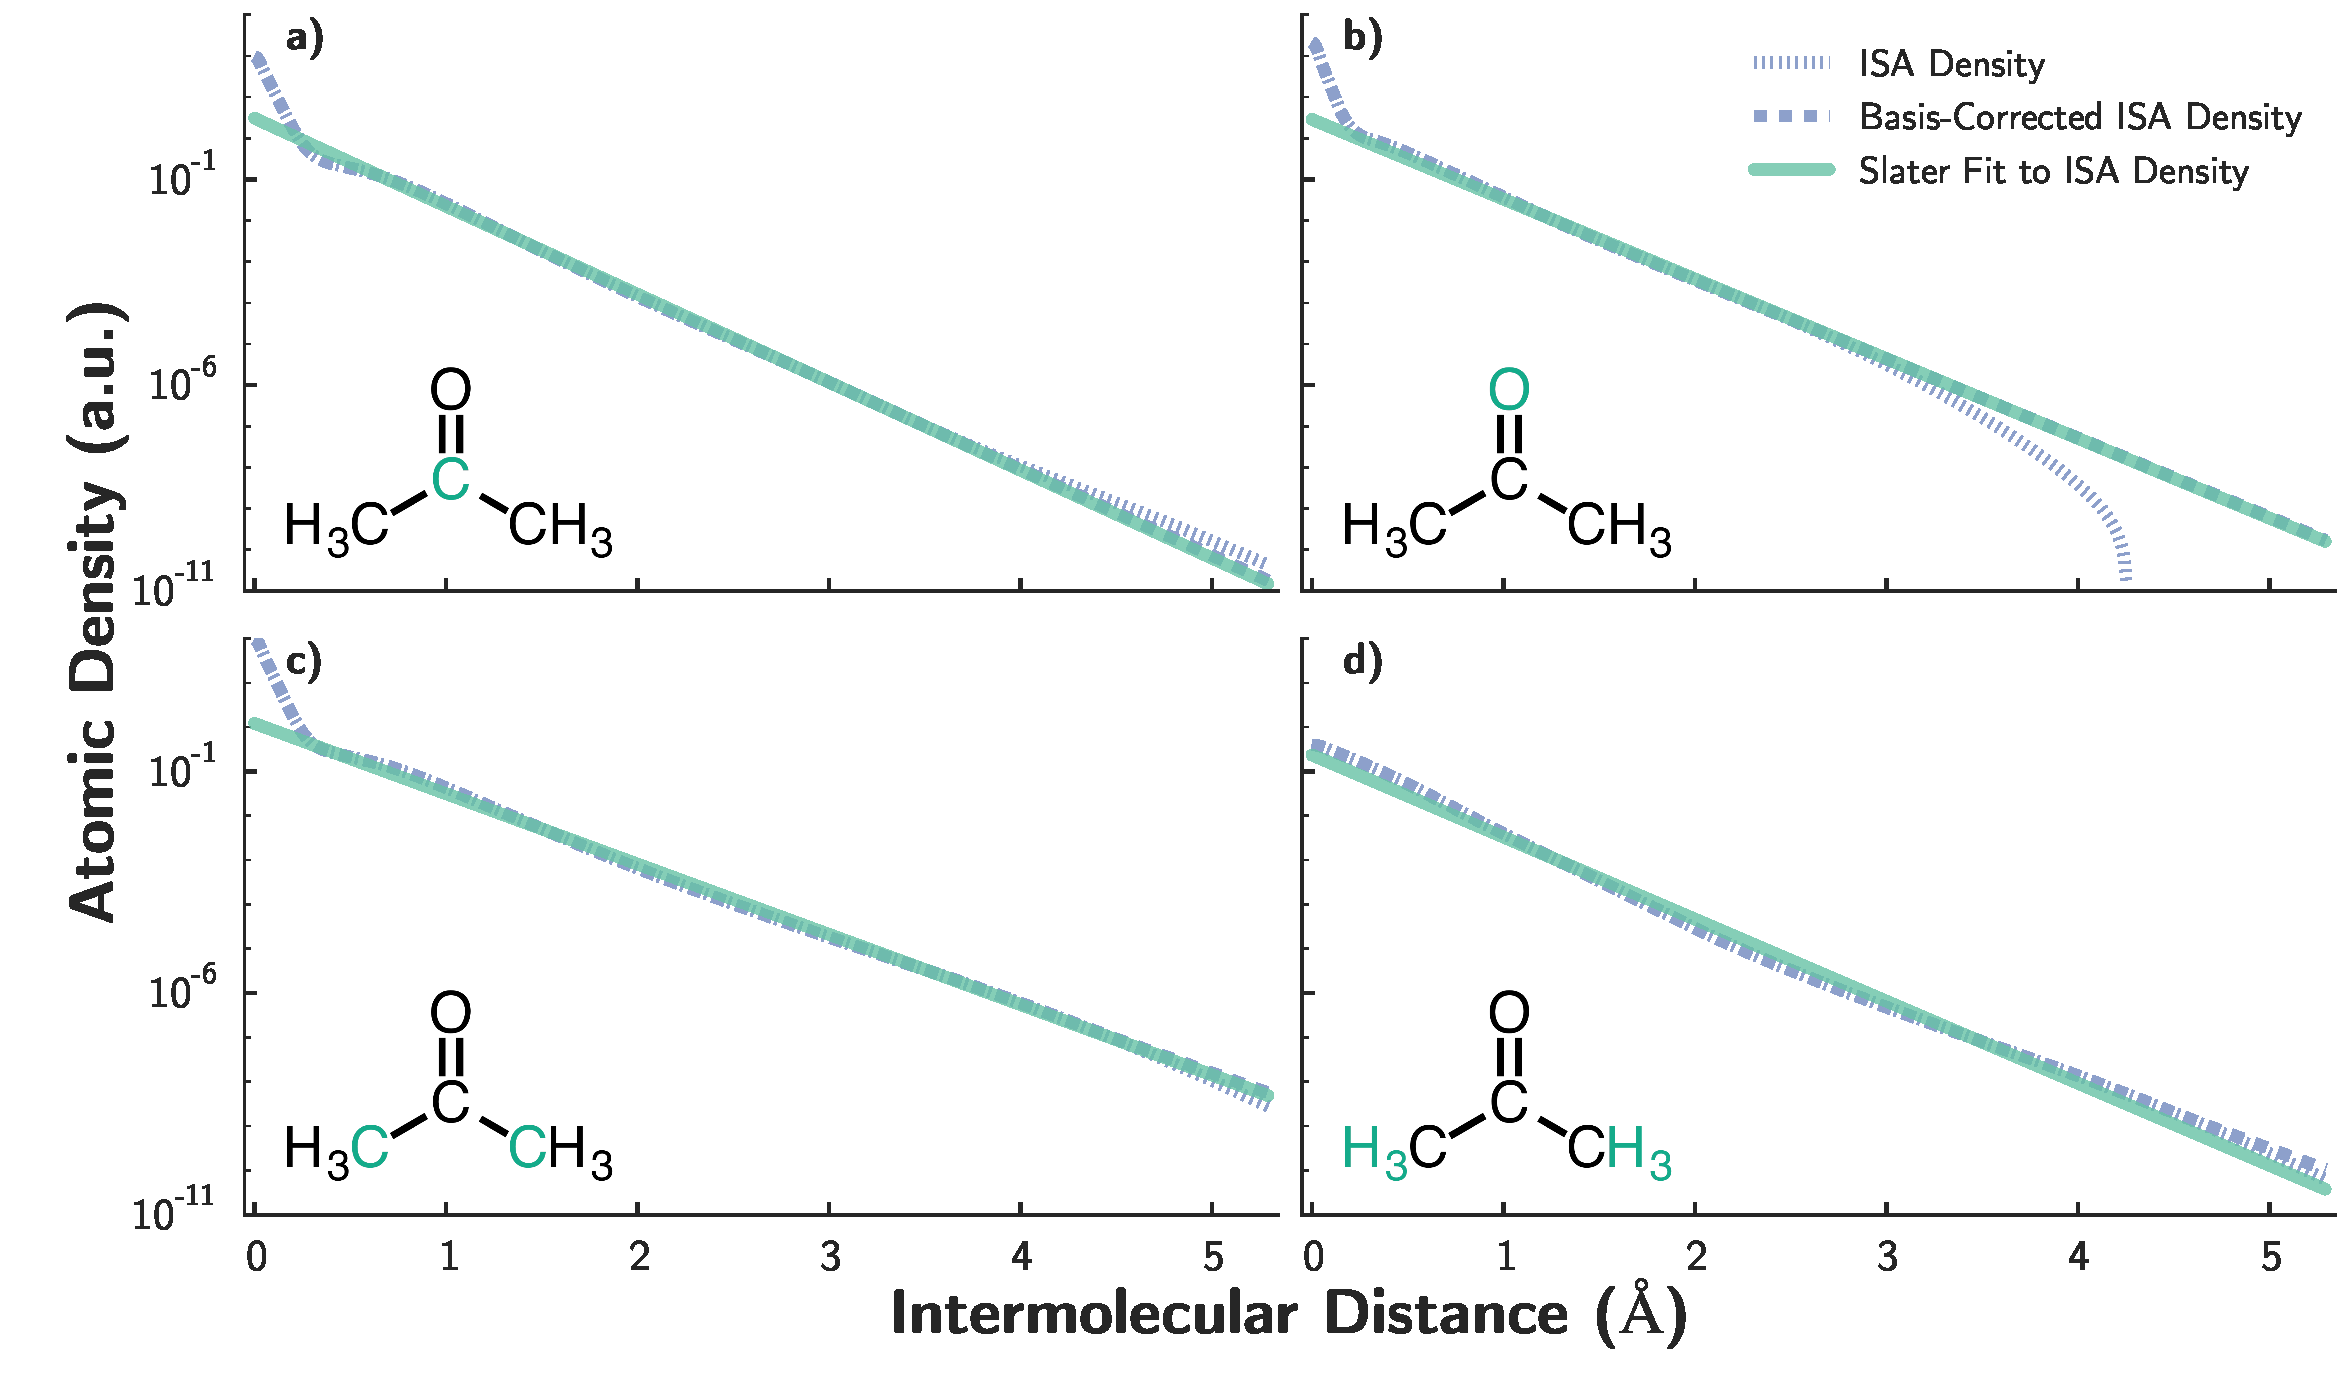
\includegraphics[width=0.9\textwidth]{isotropic/acetone_isa.pdf}  
    \caption{
        \bsisa and fitted shape functions for each atom type in acetone: a) carbonyl carbon,
        b) oxygen, c) methyl carbon, d) hydrogen. \bsisa shape functions (dotted line)
        for each atom type have been obtained at a
        PBE0/aug-cc-pVTZ level of theory. A modified \bsisa shape
        function (dashed line) corrects the tail-region of the \bsisa function to
        account for basis set deficiencies in the \bsisa algorithm. A single Slater
        orbital of the form $D_i^{\text{ISA}}\exp(-\Bisa{i} r)$ (solid line) is fit to the basis-corrected
        \bsisa shape function, and the obtained $\Bisa{i}$ value is used as an atomic exponent
        in the functional form of \isaff. Results for acetone are typical of
        molecules studied in this Chapter.
    		   }
    \label{fig:isotropic-bsisa}
    \end{figure}
    %%%%%%%%% Acetone-ISA %%%%%%%%%%%%%%%%%%%%

%ASK: Change 'basis-corrected' to 'tail-corrected?'
From \cref{fig:isotropic-bsisa} we see that the ISA atomic shape functions (that is, the
spherically-averaged ISA atoms-in-molecule density) 
decay exponentially outside the core region.
However, note that the exponents governing the spherical density decay, $\Bisa{i}$, 
differ from those of the free atoms. The ISA densities have been observed to account
for electron movement in the molecule, and the consequent density changes
brought about by this movement tend to be manifested in the region of the 
density tails. \cite{Misquitta2014}
The ISA exponents can be obtained by a weighted least-squares fit to the \bsisa atomic density
(see \cref{sec:isotropic-methods} for details), with the resulting fitted
atomic densities shown in \cref{fig:isotropic-bsisa}. 
Note that even a single exponential is remarkably successful in reproducing the
entirety of the valence atomic density.

Given these fitted ISA exponents, we can now apply
our short-range interaction formalism to polyatomics,
%
\begin{align}
\label{eq:isotropic-isaff_sr}
\begin{split}
V^{sr} &= \sum\limits_{ij} \Asr{ij} P(B_{ij}, r_{ij}) \exp(-B_{ij}r_{ij}) \\
P(B_{ij},r_{ij}) &= \frac13 (B_{ij} r_{ij})^2 + B_{ij} r_{ij} + 1 \\
    \Asr{ij} &= \Asr{i}\Asr{j} \\
    \B &= \sqrt{\Bisa{i}\Bisa{j}} \\
\end{split}
\end{align}
%
where the molecular
short-range energy is now a sum of atom-atom contributions. In conjunction
with appropriately damped atomic dispersion (\cref{eq:isotropic-ttdamp,eq:isotropic-isaff_ttdamp}), \cref{eq:isotropic-isaff_sr}  completely defines our new
short-range force field. We refer to this new functional form and set of atomic
exponents as the \isaff.

\end{subsection}
